
\lstset{
    language=Java,
    basicstyle=\small\ttfamily,
    keywordstyle=\color{blue},
    commentstyle=\color{gray},
    stringstyle=\color{green},
    breaklines=true
}


\chapter{Merge Funzioni di Verefoo} \label{ch:MergeChapter}

All'interno di questo capitolo verrà descritto il processo di ricerca e di sviluppo che è stato svolto per poter raggiungere il secondo macro obiettivo di questa tesi, ovvero 
la creazione di una nuova versione di Verefoo che sia in grado di istanziare, in un'unica iterazione, sia dei Firewall configurati per agire da Packet Filter che dei VPN Gateway 
che permettono la comunicazione cifrata fra due endpoints.\\
Il lavoro prodotto al fine di raggiungere questo obiettivo pur essendo sufficiente è tuttavia non pienamente completo per garantire una versione di Verefoo priva di errori di correttezza delle soluzioni prodotte,
ma garantisce una prima versione stabile e parzialmente corretta dell'implementazione. Durante gli studi e lo sviluppo del Merge delle due versioni sono infatti state eseguite numerose prove 
per garantire un merge che mantenesse quanto più possibile le peculiarità delle versioni utilizzate precedentemente cercando di ridurre al minimo i problemi verificatisi durante l'implementazione.\\
Nei paragrafi seguenti verrà descritto il processo di sviluppo che è stato effettuato per ottenere la versione più stabile possibile e che minimizzasse gli errori di output possibili. Inizialmente 
verrà descritta la soluzione ibrida che si è tentato di raggiungere evidenziando le motivazioni del perchè non fosse efficiente, successivamente invece saranno illustrate due soluzioni possibili all'obiettivo
da raggiungere elencando le motivazioni che hanno portato alla scelta di una delle due soluzioni. Infine verrà mostrato brevemente con degli snippet di codice Java il funzionamento generale della versione di 
Verefoo prodotta. 

\newpage

\section{Versione Ibrida con doppio Jar File}
Il primo approccio tentato per raggiungere l'obiettivo è stato quello di utilizzare le due versioni distinte di Verefoo contemporaneamente, creando una soluzione che richiedesse due iterazioni del framework con diversi input.\\
Scendendo nel dettaglio, questa soluzione richiede lo svolgimento dei seguenti passaggi:

\begin{enumerate}
    \item \textbf{Suddivisione dei security requirements}: Il file di input che un'utente definisce per ottenere una configurazione di rete desiderata tendenzialmente contiene
        contemporaneamente sia requisiti di isolamento e raggiungibilità che requisiti di protezione. Di conseguenza è necessario suddividere i requisiti in input in due gruppi, 
        il primo contenente i requisiti necessari per la definizione dei Firewall nella topologia(ovvero isolamento e raggiungibilità) ed il secondo contenente i requisiti per la 
        definizione dei VPN Gateway (ovvero protezione). Per costruire quindi il primo input verrà mantenuta la topologia di rete eliminando uno 
        dei due gruppi di requirements dall'input iniziale.
    \item \textbf{Iterazione della prima versione di Verefoo}: Ottenuto il primo file di input è possibile eseguire il primo jar file contenente la versione di verefoo che alloca univocamente 
        i Firewall o i VPN Gateway. In questa fase è necessario utilizzare il pacchetto curl(\ref{sec:Installer}) per eseguire una chiamata API di tipo POST passando come argomento della chiamata l'input 
        prodotto al punto precedente. La chiamata restituirà un output nel quale i Firewall o i VPN Gateway saranno allocati(a seconda della versione utilizzata per prima), ove necesario, al posto degli allocation places disponibili mentre tutti gli allocation
        places aggiuntivi verranno sostituiti da dei semplici forwarder. 
    \item \textbf{Traduzione Output prima versione e creazione del nuovo input}: L'output prodotto nel passaggio precedente non è utilizzabile per la seconda iterazione di Verefoo. Risulta quindi necessario
    \   tradurlo in una versione comprensibile da Verefoo. I nodi dove sono state allocate Network Security Functions verranno mantenute nell nuovo input, assieme all'inseme di nodi definiti precedentemente. Tutti i nodi
        che erano invece stati trasformati da allocation places a forwarder devono essere ritradotti come allocation places, ed infine il secondo gruppo di requirements deve essere aggiunto alla descrizione del grafo di input.
    \item \textbf{Iterazione della seconda versione di Verefoo}: Una volta terminata la produzione del secondo input è possibile eseguire il secondo file jar che si occupa dell'allocazione della Network
        Security Function rimanente in base alla scelta effettuata al punto 2. Come fatto precedentemente viene quindi eseguita una chiamata API di tipo POST tramite il pacchetto curl passando come argomento della chiamata
        il secondo input prodotto. Il risultato definito in output rappresenta la topologia di rete che l'utente ha richiesto soddisfacendo contemporaneamente sia i requisiti di raggiungibilità ed isolamento che i requisiti di protezione.
\end{enumerate}

Seppur teoricamente questa soluzione sembra un buon tentativo primitivo di risolvere il problema delle versioni multiple con Verefoo, 
essa presenta numerose limitazioni e difficoltà che ne hanno reso impossibile la realizzazione.
\\ \\
Uno degli ostacoli principali è stata la traduzione del primo output nel secondo input descritta al punto 3. Infatti Verefoo non fornisce un metodo per comprendere in maniera univoca quali sono i Forwarder presenti nella rete precedentemente all'allocazione
delle Network Security Functions rispetto a quelli che vengono tradotti successivamente al non utilizzo di un allocation places. Questo rende praticamente impossibile creare un software che traduca automaticamente l'output fornito dalla 
prima iterazione in un input idoneo per la seconda iterazione, non rendendo questa soluzione automatizzabile. Inoltre, delegare all'utente la configurazione del secondo file manualmente reintrodurrebbe la variabile di errore umano per cui Verefoo è stato sviluppato
vanificando l'intero lavoro.
\\ \\
In seconda battuta è stato analizzato quale delle due versioni del framework andasse utilizzata per la prima chiamata API(step 2) e quale per la seconda(step 4). Sebbene la scelta possa sembrare indifferente, a livello implementativo potrebbe portare a delle computazioni più complesse a causa delle operazioni che le NSFs
svolgono all'interno della topologia. I firewall per agire da packet filter devono infatti ispezionare i pacchetti che transitano attraverso il nodo e questo va in diretta contrapposizione con i tunnel VPN che vengono istanziati. Se infatti viene allocato un tunnel VPN nel quale path è presente un firewall questo non sarà in
grado di poter ispezionare il pacchetto essendo completamente incapsulato dal protocollo ESP di IPsec.
\\ \\ 
Come ultima criticità di questa soluzione, che ha portato la ricerca di una soluzione alternativa, è stata la vera e propria incompatibilità delle due versioni del framework. Scendendo più nel dettaglio, è stato notato come pur traducendo momentaneamente manualmente il primo output in un input elegibile per la seconda versione di 
Verefoo quest'ultimo continuava a non trovare una soluzione ottimale o in alcuni casi addirittura a dare errore di computazione restituendo un \textit{"503: Internal Server Error"} come risposta alla POST effettuata. Indagando è emerso che la versione che si occupava di Firewall non poteva in alcun modo accettare un input contenente
dei Gateway VPN in quanto questi non erano stati definiti all'interno del codice del file jar e di conseguenza non venivano riconosciuti come Network Security Functions. Viceversa anche allocando prima i Firewall e successivamente i Gateway VPN la soluzione non veniva comunque computata in quanto, seppur presente la definizione dei Firewall all'interno del file Jar,
i vincoli utilizzati per definire il problema MaxSMT riguardanti i Firewall non erano aggiornati allo stato più recente della ricerca, andando in conflitto con i nuovi security requirements in input.\\
Di conseguenza lo sviluppo di questa soluzione si è interrotto privilegiando una soluzione che prevedesse un'unica iterazione per l'allocazione di entrambe le Network Security Function.

\section{Versioni Firewall-to-VPN e VPN-to-Firewall}

Dovendo sviluppare una soluzione univoca una delle prime scelte effettuate è stata la decisione di cosa dover allocare in maniera prioritaria fra Firewall e VPN Gateway.
Inizialmente si è preferito optare per una soluzione nella quale i Firewall venissero allocati prima dei Gateway VPN, in quanto la versione di Verefoo contentente l'allocazione e la configurazione dei Firewall era considerabile come la versione più aggiornata e testata rispetto alle altre e quindi un'ottima base di partenza per il lavoro di sintesi delle versioni.\\
Tuttavia questa scelta è stata celermente scartata in quanto avere una soluzione intermedia nella quale sono già presenti i Firewall rispetto alle VPN porta a due problemi principali:

\begin{enumerate}
    \item \textbf{Firewall all'interno dei Tunnel VPN}: Potrebbe capitare che il firewall non riesca a svolgere la sua funzione allocandolo precedentemente ai gateway VPN. Infatti è possibile che il framework
        inserisca nel path di alcuni pacchetti che devono essere scartati dal firewall dei tunnel VPN che ovviamente, per garantire l'integrità dei dati, cifreranno il pacchetto e modificheranno il proprio header
        inserendo come IPsrc e IPdst i due estremi del VPN Gateway. Se tali pacchetti dovessero passare da un firewall configurato precedentemente per bloccare determinati pacchetti provenienti con un IP diverso da quello di incapsulamento 
        potrebbe capitare che il pacchetto attraversi il tunnel senza venir scartato.
    \item \textbf{Maggiore calcolo computazionale}: Allocare precedentemente un Firewall richiede un calcolo medio computazionale maggiore, perchè nella successiva allocazione dei Gateway VPN il framework dovrà trovare, al minimo, 2 nodi 
        di tipo allocation places disponibili per poter istanziare un tunnel. Viceversa invece istanziando precedentemente un tunnel VPN servirà solo 1 nodo per l'allocazione del firewall, rendendo la ricerca nello spazio delle soluzioni possibili
        più rapida e computazionalmente leggera.
\end{enumerate}

Considerando queste due motivazioni è stato quindi deciso di utilizzare univocamente soluzioni del tipo VPN-to-Firewall rispetto a quelle Firewall-to-VPN.\\
Tuttavia, per futuri lavori, le soluzioni Firewall-to-VPN non sono da escludere a priori in quanto è possibile realizzarle senza che entrino in conflitto con i Firewall, ma per 
garantire ciò è fondamentale che le configurazioni del firewall vengano sovrascritte tenendo conto di eventuali tunnel VPN che il framework potrebbe allocare, modificando le regole del firewall con i nuovi indirizzi IP del tunnel. Per fare ciò tuttavia è necessario modificare
diverse features di Verefoo che non sono state argomento di approfondimento nello svolgimento di questo lavoro di tesi e perciò questa possibilità viene delegata al prossimo studio di implementazioni di soluzioni miste.
\\
Un altro elemento che è stato materia di studio all'interno dello sviluppo di questa soluzione è stata l'analisi della disponibilità dei singoli allocation places per la ricerca di soluzioni ottimali.
Più precisamente, essendo la collocazione delle network security functions suddivisa per ogni funzione di rete è possibile trovarsi nella situazione in cui un allocation places che sarebbe stato un candidato ideale per la collocazione di una funzione di sicurezza viene occupato
precedentemente da un'altra funzione di sicurezza. Questa situazione potrebbe portare quindi non solo a delle soluzioni che si possono definire sub-ottimali ma anche a delle situazioni limite in cui gli allocation places non sono sufficienti rispetto al numero di Network Security Functions
che devono essere istanziate nella topologia di rete. Di seguito viene rappresentato un esempio molto semplice di caso limite che mostra questa circostanza: 

\begin{figure}[h]  % 'h' significa che la figura viene posizionata qui
    \centering
    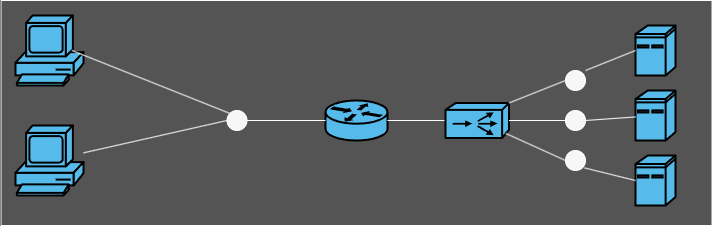
\includegraphics[width=1\textwidth]{CasoLimite.png}  % Sostituisci 'nome_immagine' con il nome del tuo file immagine e l'estensione
    \caption{Definizione esempio caso limite per duplice allocazione}
    \label{fig:CasoLimite1}
\end{figure}

All'interno di questo esempio l'utente vuole creare una rete nella quale solo uno dei due Web Client a sinistra possa comunicare con i Web Server a destra mentre l'altro Web Client,
che possiamo definire "client zombie" deve essere completamente isolato dal resto della topologia di rete. Inoltre viene richiesto che il collegamento fra uno dei tre server ed il Web Client
sia protetto, e quindi il traffico che transita per quello specifico percorso deve venire cifrato da un endpoint all'altro.\\
In questo caso allocando prima i VPN gateway per garantire i requisiti di protezione il risultato che ci si aspetta è il seguente:


\begin{figure}[h]  % 'h' significa che la figura viene posizionata qui
    \centering
    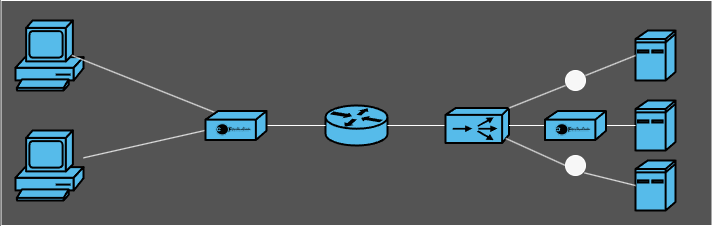
\includegraphics[width=1\textwidth]{CasoLimite2.png}  % Sostituisci 'nome_immagine' con il nome del tuo file immagine e l'estensione
    \caption{Allocazione parziale del caso limite}
    \label{fig:CasoLimite2}
\end{figure}

I gateway, seppur istanziati correttamente, fanno emergere chiaramente un grande problema, ovvero che al fine di poter rispettare anche i requisiti di
isolamento il numero di allocation point definiti inizialmente non è sufficiente all'interno dell'input fornito dall'utente. Inoltre se fossero stati allocati
i Firewall precedentemente alle VPN si sarebbe arrivati ad una situazione speculare nel momento in cui sarebbe stato necessario allocare i gateway.\\
Al fine di proporre una soluzione valida a questo problema, è stato deciso di inserire un ulteriore passo durante l'allocazione delle prime Network Security Functions,
ovvero di istanziare, contestualmente alla funzione corrente, altri N allocation places, uno per ogni nodo adiacente alla singola Network Function istanziata nell'allocation place 
scelto. Riprendendo l'esempio precedente l'output parziale prodotto dal framework sarà il seguente:


\begin{figure}[h]  % 'h' significa che la figura viene posizionata qui
    \centering
    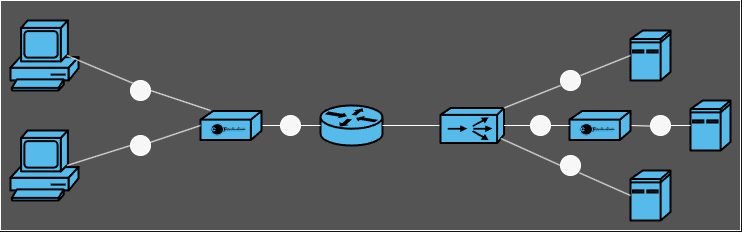
\includegraphics[width=1\textwidth]{CasoLimite3.png}  % Sostituisci 'nome_immagine' con il nome del tuo file immagine e l'estensione
    \caption{Soluzione all'allocazione parziale del caso limite}
    \label{fig:CasoLimite3}
\end{figure}
Attraverso l'introduzione di ulteriori allocation places la topologia risulterà più complessa, ma allo stesso tempo verrà concessa a Verefoo la possibilità di avere uno spazio di soluzioni
possibili per risolvere l'input fornito maggiore. Di conseguenza la soluzione ottimale che verrà prodotta sarà non solo possibile nel caso limite, ma anche tendenzialmente migliore delle precedenti
nei casi più comuni, in quanto sarà possibile applicare le restrizioni di sicurezza in più punti della rete intervenendo prima sui pacchetti che necessitano di essere scartati ma anche posizionando 
i vari gateway VPN in posizioni più strategicamente valide all'interno della topologia. Infine viene fornito, nella figura sottostante, la soluzione finale che Verefoo produrrà in output per il caso
descrito in questo paragrafo:

\begin{figure}[h]  % 'h' significa che la figura viene posizionata qui
    \centering
    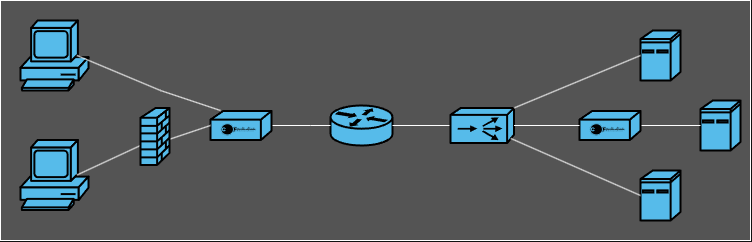
\includegraphics[width=1\textwidth]{CasoLimite4.png}  % Sostituisci 'nome_immagine' con il nome del tuo file immagine e l'estensione
    \caption{Soluzione finale caso limite}
    \label{fig:CasoLimite4}
\end{figure}


\section{Trasposizione Teorica in Codice: Analisi dell'Implementazione}
Definite le implementazioni desiderate all'interno dell'analisi delle possibili soluzioni, il framework è stato modificato adeguatamente per poter effettuare, come descritto prima, in un'unica iterazione
l'allocazione dei VPN Gateway necessari per garantire i requisiti di protezione e dei Firewall per garantire i requisiti di isolamento e raggiungibilità in questo ordine. All'interno di questo paragrafo, verranno mostrati
i punti salienti del codice al più alto livello effettuati, ovvero le classi di Verefoo che agiscono come Proxy e come Serializer. L'implementazione di più basso livello invece, allo stato precedente alle modifiche effettuate da questo lavoro, era già stato definito tramite vincoli 
descritti nella comunicazione con il Theorem Prover Z3 e tramite la definizione delle classi delle varie Network Security Functions.
Il linguaggio di sviluppo del framework è Java, pertanto il codice che verrà descritto di seguito utilizzerà
tale linguaggio di programmazione. \\
Prima di dare uno sguardo alle implementazioni delle classi è bene descrivere a grandi linee il flow chart del framework. Ad ogni esecuzione di una chiamata API Verefoo esegue le seguenti istruzioni:

\begin{enumerate}
    \item \textbf{Lettura Input e Traduzione}: Nelle primissime fasi tramite un marshaller vengono effettuate le traduzioni dell'input da un file di testo ad un file XML comprensibile e memorizzabile all'interno della memoria di Verefoo. In questa fase viene quindi effettuata 
        una validazione dell'input nelle sue varie componenti.  
    \item  \textbf{Invocazione del Serializer}: Definito l'input valido viene creata una istanza della classe del Serializer che è una classe che si occupa di "incapsulare" tutte le attività di Verefoo. Viene definito serializer perchè
        nel caso di molteplici Service Graph mandati in input esegue in maniera serializzata tutte le procedure necessarie per far lavorare Z3 correttamente per ogni grafo.
    \item \textbf{Invocazione del Normalizer}: All'interno del Serializer la prima operazione che viene effettuata è l'invocazione del Normalizer che si occupa di produrre, dato l'input fornito dall'utente e reso comprensibile con il marshaller, di produrre una versione normalizzata del grafo.
    \item \textbf{Invocazione del Proxy}: Dopo aver creato un input normalizzato viene chiamato il Proxy che si occupa di svolgere il calcolo del problema MaxSMT per produrre una soluzione.
    \item \textbf{Traduzione output}: Infine come ultimo passo, il framework traduce l'output prodotto all'interno del proxy sotto forma di file XML per renderlo più comprensibile all'utente.
\end{enumerate}

Le modifiche più significate effettuate all'interno del work flow di verefoo sono state eseguite all'interno dei file VerefooSerializer e VerefooNormalizer.
Di seguito viene fornita la nuova versione del Serializer:

\lstset{language=Java} % Imposta il linguaggio per il listing

\begin{lstlisting}[caption={Esempio di codice Java}, label=lst:java_example]
    public VerefooSerializer(NFV root) {



    int flag=0;
    this.nfv = root;
    AllocationGraphGenerator agg = new AllocationGraphGenerator(root);
    root = agg.getAllocationGraph();
    VerefooNormalizer norm = new VerefooNormalizer(root);
    root = norm.getRoot();
    try {
        List<Path> paths = null;
        if (root.getNetworkForwardingPaths() != null)
            paths = root.getNetworkForwardingPaths().getPath();
        for (Graph g : root.getGraphs().getGraph()) {
            if (root.getProfile()==null) {
                ProfileType pt = new ProfileType();
                pt.setName(ProfileNameType.HYBRID);
                    root.setProfile(pt);
            }
            List<Property> propProtection = root.getPropertyDefinition().getProperty().stream()
                    .filter(p -> p.getGraph() == g.getId()&& p.getName().name().equals("PROTECTION_PROPERTY")).collect(Collectors.toList());
            if (propProtection.size() != 0) {
                flag=1;
                VerefooProxy test = new VerefooProxy(g, root.getHosts(), root.getConnections(), root.getConstraints(),
                        propProtection, paths, root.getProfile().getName().name() ,"VPN");

                long beginAll = System.currentTimeMillis();
                VerificationResult res = test.checkNFFGProperty();
                long endAll = System.currentTimeMillis();
                resultChecker = endAll - beginAll;

                //logger.debug("Only checker: " + (endAll - beginAll) + "ms");
                //System.out.println("Only checker: " + (endAll - beginAll) + "ms");
                time = (int) res.getTime();
                if (res.result != Status.UNSATISFIABLE && res.result != Status.UNKNOWN) {
                    //System.out.println("RAW MODEL: " + res.model.toString() );
                    Translator t = new Translator(res.model.toString(), root, g, test.getAllocationNodes(), test.getTrafficFlowsMap(),"VPN");
                    z3Model = res.model.toString();
                    t.setNormalizer(norm);
                    result = t.convert();
                    root = result;
                    sat = true;
                } else {
                    sat = false;
                    result = root;
                }
                root.getPropertyDefinition().getProperty().stream().filter(p -> p.getGraph() == g.getId())
                        .forEach(p -> p.setIsSat(res.result != Status.UNSATISFIABLE));
            }
            List<Property> prop = root.getPropertyDefinition().getProperty().stream()
                    .filter(p -> p.getGraph() == g.getId()&& (p.getName().name().equals("ISOLATION_PROPERTY")||p.getName().name().equals("REACHABILITY_PROPERTY"))).collect(Collectors.toList());

            if(propProtection.size()!=0){
                for(Property p:propProtection){
                    prop.add(createProperty(p));

                }
            }

            if(prop.size()!=0 && sat)
            {
                ServiceGraph serviceGraph= new ServiceGraph(root);
                root=serviceGraph.addAP();

                VerefooProxy test = new VerefooProxy(g, root.getHosts(), root.getConnections(), root.getConstraints(),
                        prop, paths, root.getProfile().getName().name() ,"FW");
                long beginAll = System.currentTimeMillis();
                VerificationResult res = test.checkNFFGProperty();
                long endAll = System.currentTimeMillis();
                resultChecker = endAll - beginAll;
                time = (int) res.getTime();
                if (res.result != Status.UNSATISFIABLE && res.result != Status.UNKNOWN) {
                        //System.out.println("RAW MODEL: " + res.model.toString() );
                    Translator t = new Translator(res.model.toString(), root, g, test.getAllocationNodes(), test.getTrafficFlowsMap(),"FW");
                    z3Model = res.model.toString();
                    t.setNormalizer(norm);
                    result = t.convert();
                    root = result;
                    sat = true;
                    serviceGraph.RemoveAP();
                } else {
                    sat = false;
                    result = root;
                }
                root.getPropertyDefinition().getProperty().stream().filter(p -> p.getGraph() == g.getId())
                        .forEach(p -> p.setIsSat(res.result != Status.UNSATISFIABLE));

                flag=1;
            }

            if(flag==0)
                throw new BadGraphError("No property defined for the Graph " + g.getId(),
                        EType.INVALID_PROPERTY_DEFINITION);

            //TranslatorStrongSwan translatorStrongSwan= new TranslatorStrongSwan();
            //translatorStrongSwan.translationConf(root);
        }
    } catch (BadGraphError e) {
        throw e;
    }
}

    \end{lstlisting}
    
\newpage
    \begin{lstlisting}[caption={Esempio di codice Java}, label=lst:java_example]
 
        public VerefooProxy(Graph graph, Hosts hosts, Connections conns, Constraints constraints, List<Property> prop,
        List<Path> paths, String profile,String type) throws BadGraphError {
    this.profile=profile;
    this.type=type;
    // Initialitation of the variables related to the nodes
    allocationNodes = new HashMap<>();
    nodes = graph.getNode();
    nodes.forEach(n -> allocationNodes.put(n.getName(), new AllocationNode(n)));
    wildcardManager = new WildcardManager(allocationNodes);
    properties = prop;
    securityRequirements = new HashMap<>();
    int idRequirement = 0;
    for(Property p : properties) {
        securityRequirements.put(idRequirement, new SecurityRequirement(p, idRequirement));
        idRequirement++;
    }
    
    this.paths = paths;
    this.nodeMetrics = constraints.getNodeConstraints().getNodeMetrics();
    
    //Creation of the z3 context
    HashMap<String, String> cfg = new HashMap<String, String>();
    cfg.put("model", "true");
    ctx = new Context(cfg);
            
    //Creation of the NetContext (z3 variables)
    nctx = nctxGenerate(ctx, nodes, prop, allocationNodes);
    nctx.setWildcardManager(wildcardManager);


    trafficFlowsMap = generateFlowPaths();
    allocationManager = new AllocationManager(ctx, nctx, allocationNodes, nodeMetrics, prop, wildcardManager,type);
    allocationManager.instantiateFunctions();
    allocateFunctions();
    distributeTrafficFlows();
    allocationManager.configureFunctions(type);
    check = new Checker(ctx, nctx, allocationNodes);

    formalizeRequirements();
    
}
    \end{lstlisting}



